\documentclass[11pt,a4paper]{article}

\usepackage[french]{babel}
\usepackage{fontspec}
\usepackage{geometry}
\usepackage{graphicx}
\usepackage{booktabs}
\usepackage{xcolor}
\usepackage{hyperref}
\usepackage{enumitem}
\usepackage{titlesec}
\usepackage{fancyhdr}
\usepackage{caption}
\usepackage{float}
\usepackage{microtype}
\usepackage{setspace}

\geometry{margin=2.3cm}
\setmainfont{Segoe UI}
\setmonofont{Consolas}[Scale=0.9]

\definecolor{tspblue}{RGB}{0,70,127}

\hypersetup{colorlinks=true, linkcolor=tspblue, urlcolor=tspblue}

\titleformat{\section}{\Large\bfseries\color{tspblue}}{\thesection.}{0.5em}{}
\titleformat{\subsection}{\normalsize\bfseries}{\thesubsection.}{0.4em}{}
\titlespacing*{\section}{0pt}{1.2em}{0.55em}

\pagestyle{fancy}
\fancyhf{}
\fancyhead[L]{\small CSC 8607 -- TP4}
\fancyhead[R]{\small Nassim EL HADDAD}
\fancyfoot[C]{\thepage}
\renewcommand{\headrulewidth}{0.3pt}

\captionsetup{font=small, labelfont=bf}
\setlist[itemize,enumerate]{leftmargin=1.3em, itemsep=0.2em, topsep=0.3em}
\onehalfspacing

\begin{document}

\begin{center}
  {\LARGE\bfseries TP~4 -- Réseaux récurrents}\\[0.35cm]
  {\large Génération de partitions ABC}\\[0.35cm]
  {\large CSC 8607}\\[0.6cm]
  Nassim EL HADDAD
\end{center}
\vspace{0.4cm}

\section{Exploration et prétraitement}

Le corpus utilisé est constitué de partitions musicales au format ABC.
Il contient \textbf{214\,122 partitions d'entraînement} et
\textbf{2\,162 partitions de validation}.
Le vocabulaire, construit au niveau caractère, comporte
\textbf{95 symboles différents}.
Les partitions d'entraînement ont une longueur moyenne de
\textbf{290,1 caractères}, avec un maximum de
\textbf{2\,968 caractères}.

Les premières lignes d'une partition correspondent à ses métadonnées.
Par exemple, \texttt{X:} permet d'identifier la partition,
\texttt{L:} définit la durée de référence des notes,
\texttt{M:} indique la métrique et \texttt{K:} la tonalité.
Les notes et les barres de mesure apparaissent ensuite dans le contenu
musical.

\textbf{Pourquoi trier le vocabulaire~?}

Le vocabulaire est construit à partir d'un ensemble de caractères.
Or, un \texttt{set} Python ne garantit pas un ordre identique entre
deux exécutions. Sans tri explicite avec \texttt{sorted(...)},
l'association entre chaque caractère et son indice pourrait donc changer.

Cette association est utilisée pendant l'entraînement pour convertir
les caractères en indices, mais elle doit également rester identique
lors du chargement du modèle et de la génération. Sinon, un même indice
pourrait correspondre à un caractère différent et rendre les prédictions
incohérentes.

\textbf{Pourquoi tronquer les partitions à 500 caractères~?}

La longueur moyenne des partitions est d'environ 290 caractères.
Une longueur maximale de 500 permet donc de conserver une grande partie
de l'information utile tout en évitant de travailler systématiquement
avec la longueur maximale de 2\,968 caractères.

Utiliser directement cette longueur maximale augmenterait fort
le coût de la BPTT et la mémoire GPU. Les partitions courtes
devraient aussi être remplies de beaucoup de padding, ce qui
pèserait trop dans le calcul de la loss.

\section{Dataset auto-régressif et modèles}

Avec \texttt{SEQ\_LENGTH=500}, chaque partition est soit tronquée,
soit complétée par du padding afin d'obtenir une longueur fixe de
500 caractères. Le principe du dataset auto-régressif consiste ensuite
à décaler la séquence d'un caractère : \texttt{x} contient les
499 premiers caractères et \texttt{y} les 499 caractères suivants.

Avec un batch de 128 partitions, les tenseurs transmis au modèle ont
donc une forme $(128,499)$. Les données sont stockées en
\texttt{torch.long}, car elles représentent des indices de caractères.
Ce type est requis par \texttt{nn.Embedding} et
\texttt{CrossEntropyLoss}.

\textbf{Nombre de paramètres}

Pour $V=95$, $E=256$ et $H=512$, l'embedding contient
$V\times E=24\,320$ paramètres. Le bloc RNN contient $394\,240$
paramètres et la couche linéaire finale $48\,735$ paramètres, soit un
total de \textbf{467\,295 paramètres} pour le modèle RNN.

Pour le LSTM, le bloc récurrent contient quatre fois plus de
paramètres, soit $1\,576\,960$. Le LSTM utilise quatre portes,
chacune avec ses matrices et ses biais. Au total, le modèle LSTM
compte \textbf{1\,650\,015 paramètres}.

\begin{table}[H]
\centering
\small
\caption{Nombre de paramètres ($V=95$, $E=256$, $H=512$).}
\begin{tabular}{@{}lrrr@{}}
\toprule
Architecture & Embedding & Bloc récurrent & FC / Total \\
\midrule
RNN & 24\,320 & 394\,240 & 48\,735 / \textbf{467\,295} \\
LSTM & 24\,320 & 1\,576\,960 & 48\,735 / \textbf{1\,650\,015} \\
\bottomrule
\end{tabular}
\end{table}

Une couche \texttt{nn.Embedding} convient bien ici. Les indices des
caractères sont des catégories, sans relation numérique entre eux.
Les passer tels quels à une couche linéaire donnerait une fausse idée
de distance entre symboles. L'embedding associe chaque symbole à un
vecteur appris de façon indépendante.

Une autre différence importante entre les deux architectures concerne
leur état interne. Le RNN renvoie un état caché $h_t$, tandis que le
LSTM conserve deux états, $(h_t,c_t)$. Le \emph{cell state} $c_t$
constitue une mémoire à plus long terme, contrôlée par les différentes
portes du LSTM.

\section{Entraînement et comparaison RNN / LSTM}

Avant de calculer la \texttt{CrossEntropyLoss}, les dimensions des
tenseurs doivent être adaptées. Les logits passent de $(B,T,V)$ à
$(B\times T,V)$ et les cibles de $(B,T)$ à $(B\times T)$.
Avec $B=128$ et $T=499$, cela représente donc
$128\times499=63\,872$ prédictions de caractères.

Le clipping des gradients se fait après \texttt{backward()} et avant
\texttt{optimizer.step()} : les gradients n'existent qu'après la
rétropropagation, et il faut borner leur norme avant la mise à jour.

Les résultats obtenus sur le subset de 10\,000 partitions montrent une
nette différence entre les modèles. Le LSTM obtient les meilleures
performances, avec une \textbf{Val Loss de 0,56} et une
\textbf{accuracy de 81,9\,\%}, contre 77,3\,\% pour le RNN sans
clipping et 75,9\,\% pour le RNN avec clipping.

\begin{table}[H]
\centering
\small
\caption{Résultats à l'époque~15 (subset 10k, job \#9151).}
\begin{tabular}{@{}lccc@{}}
\toprule
Modèle & Val Loss & Val Acc & GradNorm moy. \\
\midrule
RNN sans clip & 0,72 & 77,3\,\% & 0,22 \\
RNN clip$=1$ & 0,76 & 75,9\,\% & 0,27 \\
\textbf{LSTM clip$=1$} & \textbf{0,56} & \textbf{81,9\,\%} & 0,08 \\
\bottomrule
\end{tabular}
\end{table}

\begin{figure}[H]
  \centering
  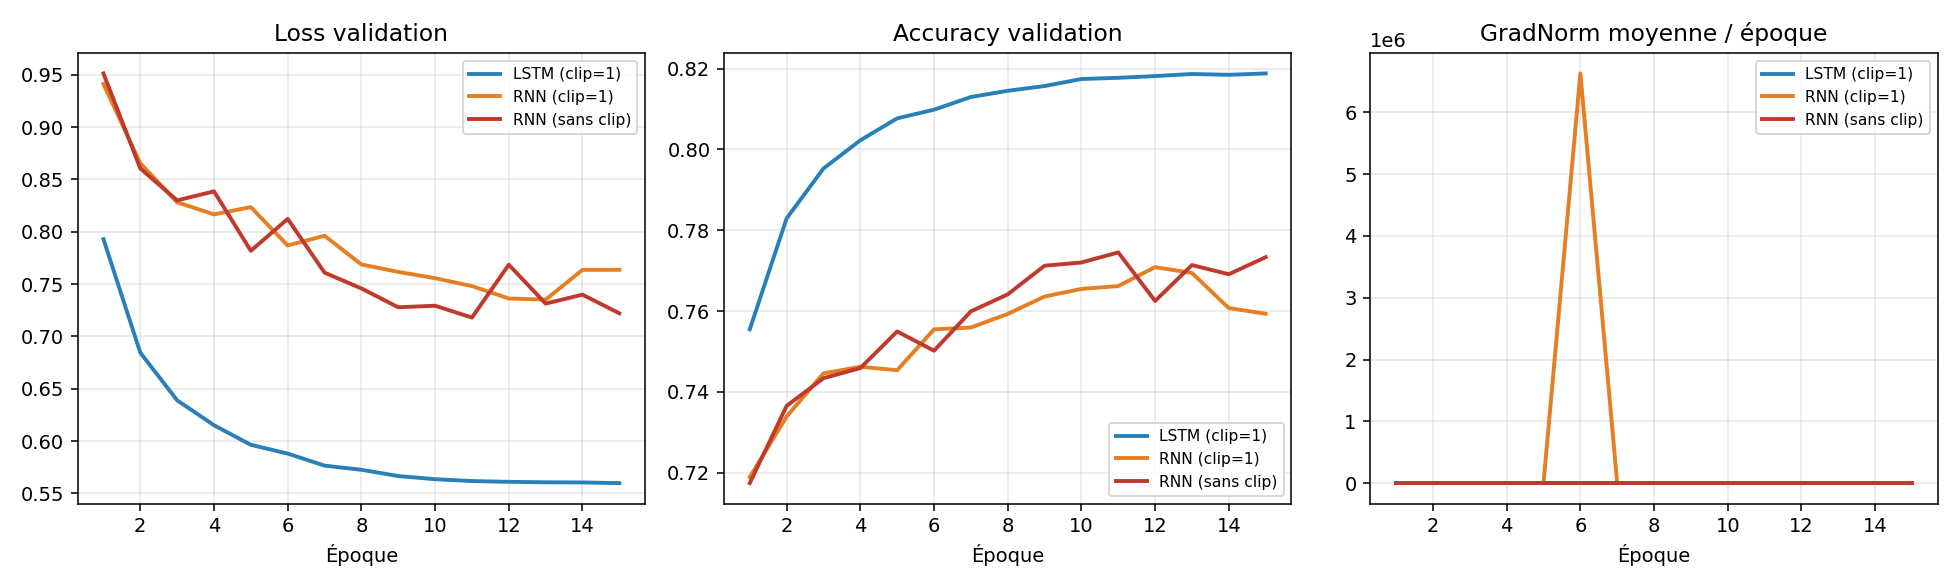
\includegraphics[width=0.98\textwidth]{figures/tb_quick_3runs.png}
  \caption{Comparaison des trois runs : loss et accuracy de validation,
  norme moyenne des gradients par époque.}
\end{figure}

\begin{figure}[H]
  \centering
  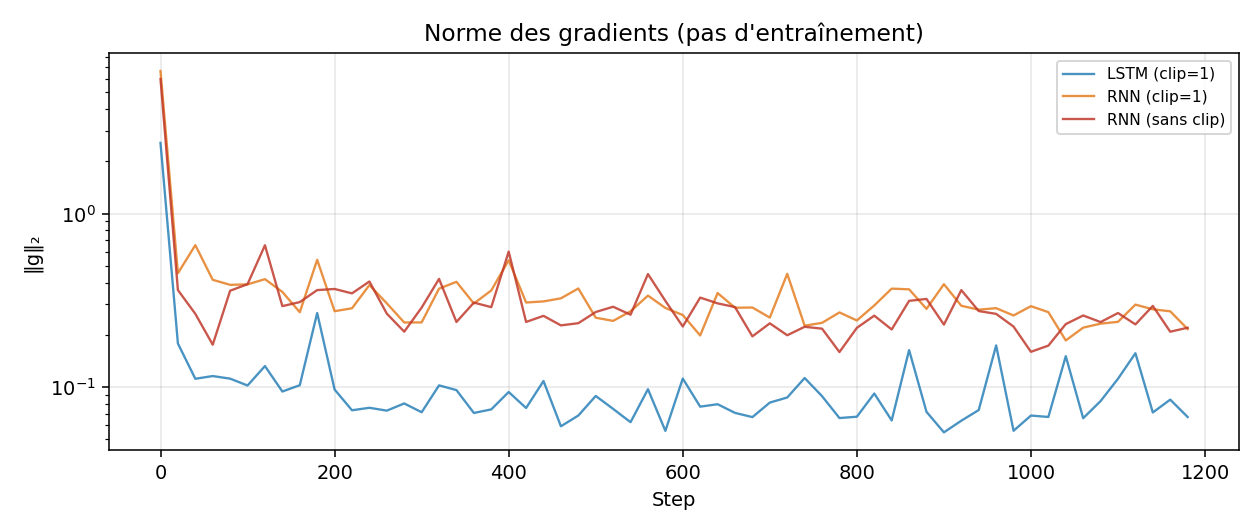
\includegraphics[width=0.92\textwidth]{figures/tb_gradnorm_step.png}
  \caption{Norme des gradients au cours des pas d'entraînement
  (échelle logarithmique).}
\end{figure}

Le clipping est surtout utile pour le RNN. Autour de la sixième époque,
la norme des gradients grimpe à plusieurs millions. C'est une
\textbf{explosion des gradients}, classique quand on rétropropage sur
de longues séquences.

La fonction \texttt{clip\_grad\_norm\_} mesure d'abord la norme, puis
la borne à la valeur choisie. Ça évite des mises à jour instables.
En revanche, le clipping ne règle pas le problème inverse : la
disparition des gradients.

Le LSTM s'en sort mieux grâce à sa mémoire. Son \emph{cell state}
suit la relation
\[
c_t = f_t \odot c_{t-1} + i_t \odot \tilde{c}_t
\]
Cette mise à jour additive laisse le gradient circuler plus facilement
sur de longues séquences. Quand la \emph{forget gate} reste proche de 1,
des informations peuvent être gardées sur beaucoup de pas. En musique,
ça aide à retenir le rythme ou des motifs apparus plus tôt dans la
partition.

L'accuracy reste à prendre avec précaution. Les partitions courtes
sont remplies jusqu'à 500 caractères : beaucoup de padding, facile à
prédire, ce qui gonfle un peu la métrique. On pourrait utiliser
\texttt{CrossEntropyLoss(ignore\_index=...)} pour ignorer ce padding
dans la loss.

\section{Génération et entraînement long}

\subsection{Complexité et température}

Lors de la génération, le modèle peut réutiliser son état caché et ne
traiter qu'un seul nouveau caractère à chaque étape. Pour générer
$N$ caractères, chaque étape étant effectuée une seule fois, la
complexité est alors en $O(N)$.

Sans réutiliser l'état caché, il faudrait à chaque étape repasser
l'ensemble de la séquence déjà générée dans le modèle. Le nombre de
calculs augmenterait alors avec la longueur de la séquence, ce qui
conduirait à une complexité en $O(N^2)$.

La température $T$ permet de contrôler le niveau d'aléatoire lors du
choix du prochain caractère. Avec une température très faible, comme
$T=0.2$, la distribution se concentre fortement sur les caractères les
plus probables. La génération devient alors plus prévisible, mais
également plus répétitive.

À l'inverse, une température élevée augmente la diversité des sorties.
Lorsque $T$ devient très grande, la distribution se rapproche d'une
distribution uniforme et les caractères moins probables sont davantage
sélectionnés. La génération devient alors plus imprévisible et peut
perdre en cohérence.

\subsection{Exemples générés}

Les exemples générés avec l'amorce \emph{Irish Reel} montrent bien
l'effet de la température. À $T=0.2$, la syntaxe ABC reste globalement
correcte, mais la sortie est très répétitive : le modèle choisit presque
toujours les caractères les plus probables.

Avec $T=0.8$, le résultat constitue un meilleur compromis entre
diversité et cohérence. Les rythmes et les enchaînements de notes sont
plus variés tout en conservant une structure musicale et syntaxique
relativement lisible.

Enfin, avec $T=2.0$, la diversité augmente fortement, mais la qualité
de la génération se dégrade. On observe davantage de caractères rares,
des en-têtes parfois incorrects et des mesures moins régulières. Une
température trop élevée favorise donc la diversité au détriment de la
validité de la partition.

\subsection{Entraînement long avec Slurm}

Un entraînement plus important a ensuite été réalisé avec un LSTM de
taille cachée $H=1024$, entraîné sur 50\,000 partitions pendant
jusqu'à 30 époques, avec un clipping des gradients à 1.

Les résultats montrent une amélioration rapide dès les premières
époques. À la sixième époque, la validation atteint une accuracy de
\textbf{83,9\,\%} avec une Val Loss de \textbf{0,50}. Les performances
sont déjà supérieures à celles obtenues avec le modèle entraîné sur le
subset de 10\,000 partitions.

\begin{table}[H]
\centering
\small
\caption{LSTM long (50k, $H=1024$, job \#9152) : premières époques.}
\begin{tabular}{@{}cccc@{}}
\toprule
Ép. & Train Loss & Val Loss & Val Acc \\
\midrule
1 & 0,76 & 0,57 & 81,3\,\% \\
2 & 0,55 & 0,53 & 82,6\,\% \\
3 & 0,51 & 0,51 & 83,2\,\% \\
4 & 0,50 & 0,50 & 83,6\,\% \\
5 & 0,48 & 0,49 & 83,8\,\% \\
6 & 0,48 & 0,50 & 83,9\,\% \\
\bottomrule
\end{tabular}
\end{table}

\begin{figure}[H]
  \centering
  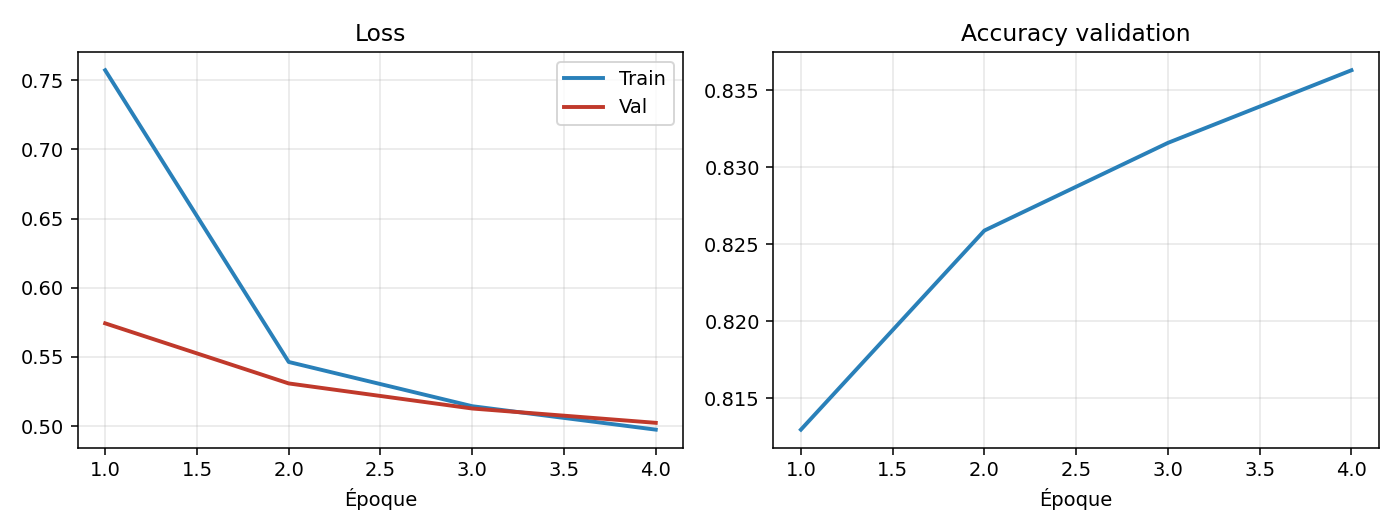
\includegraphics[width=0.92\textwidth]{figures/tb_lstm_full.png}
  \caption{Courbes du LSTM long sur 50\,000 partitions.}
\end{figure}

L'utilisation d'un corpus plus important permet donc au modèle de
disposer de davantage d'exemples et d'apprendre des représentations
plus générales de la structure musicale. Ces résultats confirment
l'intérêt d'augmenter la quantité de données disponibles pour ce type
de tâche.

\subsection{Bonus : transposition}

Une piste simple pour augmenter artificiellement la diversité du
corpus serait de transposer les mélodies d'un certain nombre de
demi-tons. Les notes ABC seraient alors décalées et la tonalité
indiquée dans l'en-tête \texttt{K:} serait adaptée en conséquence.

On garderait la structure rythmique et mélodique, tout en montrant
la même idée musicale dans plusieurs tonalités. Le modèle dépendrait
moins des tonalités dominantes du corpus, ce qui limiterait le
sur-apprentissage.

\end{document}
